\section{Resultados e Discussão}

A Tabela~\ref{tab:principal} traz o resultado de cada instância e da programação dinâmica; a Tabela~\ref{tab:bb} mostra o que o Branch-and-Bound fez em 15 minutos; as Figuras~\ref{fig:razao} e~\ref{fig:tempos} resumem a qualidade e o tempo. Todos os números vêm do arquivo \texttt{resultados.csv} do experimento, e onde os dois algoritmos terminaram os valores coincidiram.

\begin{table}[ht]\centering\footnotesize\setlength{\tabcolsep}{4pt}
\caption{Resultados nas 12 instâncias. Ótimo/melhor: ótimo provado (sem marca) ou melhor valor encontrado, sem prova de otimalidade ($^*$). Heur.: heurística do Trabalho~1. Razão: Heur./ótimo. DP: largura $w$, tempo e memória estimada (``---'': inviável, $w>26$).}\label{tab:principal}
\begin{tabular}{lrrrrcrrr}\hline
Instância & $n$ & $m$ & Ótimo/melhor & Heur. & Razão & $w$ & DP (s) & Mem. (MB) \\\hline
01\_ALE\_n100 & 100 & 200 & 168 & 158 & 0{,}940 & 21 & 0{,}173 & 26 \\
02\_ALE\_n120 & 120 & 240 & 204 & 196 & 0{,}961 & 26 & 5{,}139 & 845 \\
03\_PM1\_n120 & 120 & 240 & 83 & 69 & 0{,}831 & 26 & 5{,}147 & 845 \\
04\_TORO\_8x250 & 2000 & 4000 & 1406 & 1114 & 0{,}792 & 17 & 0{,}811 & 16 \\
05\_TORO\_10x200 & 2000 & 4000 & 1386 & 1080 & 0{,}779 & 21 & 12{,}9 & 265 \\
06\_TORO\_5x20000 & 100000 & 200000 & 69050 & 53738 & 0{,}778 & 11 & 0{,}632 & 12 \\
07\_TORO\_7x14286 & 100002 & 200004 & 69354 & 53570 & 0{,}772 & 15 & 9{,}195 & 195 \\
08\_ALE\_n200 & 200 & 400 & 322$^*$ & 316 & --- & --- & --- & --- \\
09\_PM1\_n500 & 500 & 1000 & 299$^*$ & 299 & --- & --- & --- & --- \\
10\_TORO\_20x50 & 1000 & 2000 & 528$^*$ & 516 & --- & --- & --- & --- \\
11\_G32 & 2000 & 4000 & 1170$^*$ & 1170 & --- & --- & --- & --- \\
12\_G57 & 5000 & 10000 & 2924$^*$ & 2924 & --- & --- & --- & --- \\
\hline\end{tabular}

\end{table}

\begin{table}[ht]\centering\footnotesize\setlength{\tabcolsep}{4pt}
\caption{Branch-and-Bound com limite de 900\,s. Situação: ótimo provado ou parou no limite. Nós: milhares de milhões de nós visitados. Limitante inicial: o teto \eqref{eq:ub} antes de qualquer decisão. Melhorias: quantas vezes a melhor solução encontrada melhorou.}\label{tab:bb}
\begin{tabular}{lrcrrrr}\hline
Instância & Valor & Situação & Tempo (s) & Nós ($10^9$) & Limitante inicial & Melhorias \\\hline
01\_ALE\_n100 & 168 & ótimo & 620 & 19{,}1 & 200 & 10 \\
02\_ALE\_n120 & 201 & limite & 900 & 32{,}1 & 240 & 5 \\
03\_PM1\_n120 & 75 & limite & 900 & 30{,}9 & 119 & 6 \\
04\_TORO\_8x250 & 1114 & limite & 900 & 32{,}9 & 2001 & 0 \\
05\_TORO\_10x200 & 1080 & limite & 900 & 31{,}3 & 2001 & 0 \\
06\_TORO\_5x20000 & \multicolumn{6}{c}{não executado ($n>5000$)} \\
07\_TORO\_7x14286 & \multicolumn{6}{c}{não executado ($n>5000$)} \\
08\_ALE\_n200 & 322 & limite & 900 & 35{,}9 & 400 & 6 \\
09\_PM1\_n500 & 299 & limite & 900 & 51{,}6 & 517 & 0 \\
10\_TORO\_20x50 & 528 & limite & 900 & 35{,}9 & 993 & 4 \\
11\_G32 & 1170 & limite & 900 & 34{,}4 & 2011 & 0 \\
12\_G57 & 2924 & limite & 900 & 34{,}5 & 4981 & 0 \\
\hline\end{tabular}

\end{table}

\begin{figure}[ht]
\centering
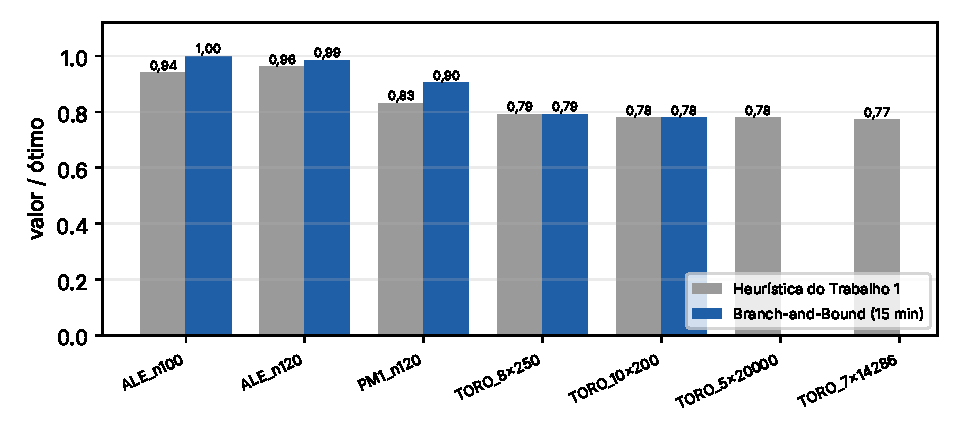
\includegraphics[width=0.92\textwidth]{fig_razao.pdf}
\caption{Valor obtido em relação ao ótimo nas instâncias em que a programação dinâmica calculou o ótimo: heurística do Trabalho~1 (cinza) e Branch-and-Bound com 15 minutos (azul). O Branch-and-Bound não roda nas instâncias de 100 mil vértices.}\label{fig:razao}
\end{figure}

\begin{figure}[ht]
\centering
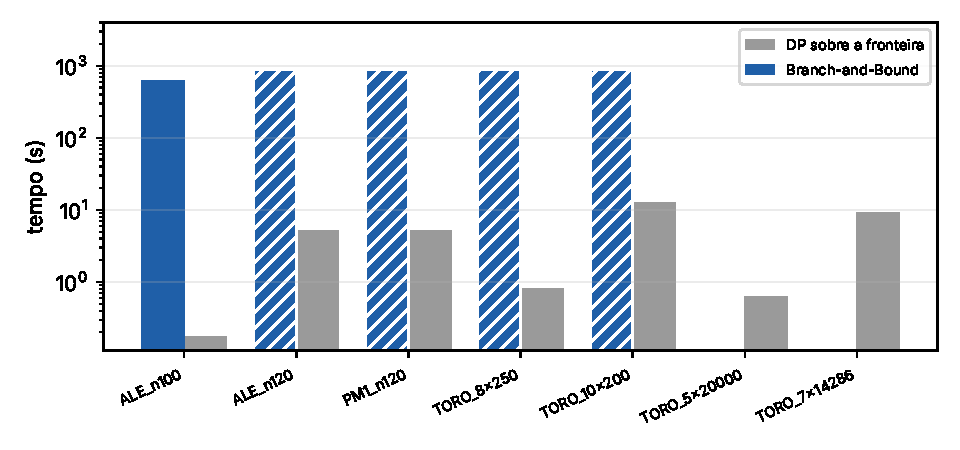
\includegraphics[width=0.92\textwidth]{fig_tempos.pdf}
\caption{Tempo do Branch-and-Bound (azul) e da programação dinâmica (cinza), em escala logarítmica. Barras hachuradas: o Branch-and-Bound parou no limite de 900\,s sem provar o ótimo.}\label{fig:tempos}
\end{figure}

\subsection{Programação dinâmica}

A programação dinâmica calculou o ótimo das 7 instâncias dos grupos A e B, inclusive as duas grades de cerca de 100 mil vértices, em 0,63\,s ($w=11$) e 9,2\,s ($w=15$). O tempo depende de $w$, e quase nada de $n$: cada 4 unidades a mais de largura multiplicam o tempo por cerca de 16 ($0{,}81$\,s com $w=17$ e $12{,}9$\,s com $w=21$, ambas com 2\,000 vértices), como previsto por $O(2^{w}(n+m))$. A memória acompanha: de 12\,MB ($w=11$) a 845\,MB ($w=26$, o limite da implementação). Nas instâncias do grupo C, a fronteira encontrada é de 41 ou mais, e a programação dinâmica não executa.

\subsection{Branch-and-Bound}

O Branch-and-Bound só provou a otimalidade de uma instância, a \texttt{01\_ALE\_n100} (ótimo 168), em 620\,s e $1{,}9\cdot10^{10}$ nós. A programação dinâmica resolve a mesma instância em 0,17\,s, cerca de 3\,600 vezes mais rápido. Nas outras 9 instâncias ele chegou ao limite de 15 minutos, depois de visitar entre 31 e 52 bilhões de nós. É um número enorme, mas pequeno diante do espaço de busca ($2^{120}$ em $n=120$; $2^{2000}$ no G32).

O motivo é que o teto é folgado. Na coluna ``Limitante inicial'' da Tabela~\ref{tab:bb}, vemos que, antes de decidir qualquer vértice, o teto já está de 18\% a 88\% acima do valor final. Nas instâncias com pesos $+1$ o teto inicial vale exatamente $m$ (200, 240 e 400): ele supõe que todas as arestas podem ser cortadas, enquanto o ótimo corta cerca de 85\% delas. Nas grades, onde metade das arestas tem peso negativo, o teto inicial é 2\,001 contra um ótimo de 1\,406 e 1\,386. Com um teto assim, só se poda quando já se perdeu muito, e isso demora a acontecer.

Mesmo assim, o Branch-and-Bound melhorou a heurística do Trabalho~1 em 5 das 10 instâncias em que roda (Figura~\ref{fig:razao}). Nas aleatórias pequenas ele chegou perto do ótimo: 168 de 168 na \texttt{01} (a heurística tinha 158), 201 de 204 na \texttt{02} (heurística 196) e 75 de 83 na \texttt{03} (heurística 69). Nas grades de 2\,000 vértices (04 e 05) não houve nenhuma melhoria em 15 minutos: o valor final é o da heurística (1\,114 e 1\,080), bem abaixo do ótimo (1\,406 e 1\,386). No grupo C, onde o ótimo é desconhecido, ele melhorou a \texttt{08} (de 316 para 322) e a \texttt{10} (de 516 para 528), e não alterou a \texttt{09}, o G32 e o G57. Como o teto inicial fica de 70\% a 73\% acima desses valores, não dá para saber se a heurística é ótima ou não nessas três: o Branch-and-Bound entrega uma solução, mas nenhuma garantia.

\subsection{Comparação com o Trabalho 1}

Com os ótimos em mãos, dá para medir a heurística do Trabalho~1 contra o valor verdadeiro. Nas grades toroidais ela obtém de 77\% a 79\% do ótimo (0,792; 0,779; 0,778 e 0,772), e a razão não piora com o tamanho: com 100 mil vértices é praticamente a mesma que com 2\,000. Nas aleatórias esparsas com pesos $+1$ ela obtém 0,94 e 0,96 (na faixa de 93\% a 96\% relatada no Trabalho~1) e, com pesos $\pm1$, 0,83. Esses valores são da mesma ordem dos 80\% a 82\% do melhor valor conhecido que o Trabalho~1 relatou nos toroidais do G-set, o que sugere que a diferença se deve sobretudo à busca local, e não a uma referência frouxa. Para o G32 e o G57 não podemos afirmar o mesmo: a versão da heurística incorporada ao programa novo dá 1\,170 e 2\,924 (0,83 e 0,84 dos melhores valores conhecidos, 1\,410 e 3\,494), um pouco acima dos 0,82 do relatório anterior. Ou seja, o desempate da ordenação por grau já move o resultado em 1\% a 3\%. O Branch-and-Bound não alterou esses dois valores.

O preço do ótimo também fica claro: a heurística leva de 8\,$\mu$s (100 vértices) a 12\,ms (100 mil vértices); a programação dinâmica, de 0,17\,s a 13\,s onde roda; e o Branch-and-Bound, 10 minutos para provar uma instância de 100 vértices e mais de 15 minutos nas demais. A heurística é a melhor escolha quando o tempo importa; os algoritmos exatos servem para medir quanto ela deixa de ganhar, que nas grades é de 21\% a 23\% do ótimo.

\subsection{Comparação com a literatura}

Não dá para comparar tempos diretamente com os resolvedores da literatura: não usamos as instâncias da \emph{Biq Mac Library} nem os códigos do \emph{Biq Mac} e do \emph{BiqCrunch}, e as máquinas são diferentes. O que podemos dizer é qualitativo. O \emph{Biq Mac} resolve qualquer instância de até 100 vértices, mesmo densa \cite{Rendl et al. 2010}; nosso Branch-and-Bound provou uma instância esparsa de 100 vértices em 10 minutos e não resolveu as de 120, o que é esperado, pois seu teto é bem mais fraco que o semidefinido. A programação dinâmica resolve aleatórios esparsos até 120 vértices em 5\,s, mas só porque são esparsos; em grafos densos seria inviável. O branch-and-cut de \citet{Liers et al. 2003} chega a 1\,280 vértices em grafos aleatórios de grau 4, uma ordem de grandeza acima do que alcançamos (a \texttt{08\_ALE\_n200} está fora do alcance da nossa programação dinâmica). Nossas grades de 100 mil vértices só são resolvidas porque a largura é pequena, e não porque o algoritmo seja mais forte.

\subsection{Limitações}

Cada instância foi executada uma vez, em uma única máquina, e há uma instância por tipo e tamanho, então os resultados mostram o comportamento, mas não são uma estatística. O limite de 900\,s é arbitrário; com mais tempo o Branch-and-Bound poderia provar alguma instância pequena a mais. A ordem da programação dinâmica é heurística, e uma ordem melhor poderia resolver instâncias maiores (nas do grupo C só estimamos a largura com poucas tentativas). Nas instâncias 08 a 12 o ótimo é desconhecido, e o valor final do Branch-and-Bound é só um limite inferior para ele.

\section{Conclusão}

Implementamos e validamos dois algoritmos exatos para o Corte Máximo, um Branch-and-Bound e uma programação dinâmica sobre a fronteira, ambos com prova de correção e análise de custo. Em 12 instâncias de 100 a 100\,002 vértices, com limite de 15 minutos por algoritmo, a programação dinâmica calculou o ótimo de 7, inclusive duas grades toroidais de cerca de 100 mil vértices (em 0,63\,s e 9,2\,s), porque a fronteira é pequena. O Branch-and-Bound provou a otimalidade de uma instância (100 vértices, 620\,s) e esgotou o tempo nas demais, porque seu teto é folgado; mesmo assim, devolveu soluções melhores que as da heurística em 5 das 10 instâncias em que roda.

Com os ótimos, confirmamos o diagnóstico do Trabalho~1: a heurística gulosa com busca local obtém de 77\% a 79\% do ótimo nas grades toroidais com pesos $\pm1$, de 2\,000 a 100 mil vértices, e de 83\% a 96\% em aleatórias esparsas pequenas. As instâncias do G-set (G32 e G57) continuam fora do alcance dos dois algoritmos.

Como trabalho futuro, o ganho mais claro está em tetos melhores para o Branch-and-Bound (por exemplo, com programação linear ou semidefinida, como a literatura faz) e em ordens melhores para a programação dinâmica. Também valeria rodar os algoritmos nas instâncias da \emph{Biq Mac Library}, para uma comparação direta com a literatura.
